\documentclass{article}
\usepackage[final]{nips_2017}
\usepackage[utf8]{inputenc} % allow utf-8 input
\usepackage[T1]{fontenc}    % use 8-bit T1 fonts
\usepackage{hyperref}       % hyperlinks
\usepackage{url}            % simple URL typesetting
\usepackage{booktabs}       % professional-quality tables
\usepackage{amsfonts}       % blackboard math symbols
\usepackage{nicefrac}       % compact symbols for 1/2, etc.
\usepackage{microtype}      % microtypography
\usepackage{graphicx}

\usepackage{mathpazo}
\usepackage{hyperref,url}
\usepackage{amsmath}
\usepackage{caption}
\usepackage{subcaption}
\usepackage{float}
\usepackage{graphicx}
\usepackage{cleveref}
\usepackage{listings}
\usepackage{subcaption}
\usepackage[font={small}]{caption}
\usepackage{listings}


%\usepackage[backend=bibtex, sorting=none]{biblatex}
%\bibliography{references}
%\AtBeginBibliography{\footnotesize}

\title{Predicting mRNA splicing levels from sequence}

\author{
  Ramya Rangan\\
  Stanford University\\
  \texttt{ramyar@stanford.edu} \\
  %% examples of more authors
  %% \And
  %% Coauthor \\
  %% Affiliation \\
  %% Address \\
  %% \texttt{email} \\
  %% \AND
  %% Coauthor \\
  %% Affiliation \\
  %% Address \\
  %% \texttt{email} \\
  %% \And
  %% Coauthor \\
  %% Affiliation \\
  %% Address \\
  %% \texttt{email} \\
  %% \And
  %% Coauthor \\
  %% Affiliation \\
  %% Address \\
  %% \texttt{email} \\
}

\begin{document}
% \nipsfinalcopy is no longer used

\begin{center}

\includegraphics[width=3cm, height=0.7cm]{../figures/CS230}
\end{center}

\maketitle

\begin{abstract}
Compared to a bi-directional LSTM and deeper CNN approach, we find that a simple CNN architecture with 1 residual block achieves best splicing efficiency predictions, with mean squared error better than the baseline model (0.102 vs 0.202).
\end{abstract}

\section{Introduction}	
\subsection{Description}
The process of accurately and efficiently creating mRNA and then proteins from our genomes' DNA is critical for nearly all biological processes. Over 95\% of human genes are edited via {\bf mRNA splicing}, a process in which large sections of mRNA known as {\bf introns} are precisely recognized and removed to create the final mature mRNA that encodes the correct protein product (Figure \ref{fig:splicing}). Errors in mRNA splicing are implicated in a host of diseases from autism to cancers, with mistakes in this editing process leading to incorrect protein products and downstream disease pathways. Splicing proceeds via the recognition of specific parts of the mRNA sequence, but the patterns are complex, with mRNA sequence features influencing protein binding and RNA structures which in turn effects splicing levels. Though it is of great interest to understand the rules that govern the extent to which splicing occurs at a particular position in mRNA, we do not yet have predictive models that can determine splicing efficiency from an mRNA's sequence. Here we explore CNN and RNN approaches for predicting splicing efficiency values ranging from 0 to 1 given a sequence of RNA nucleotides.
\begin{figure}[H]
\centering
\begin{subfigure}{.4 \textwidth}
\centering
\caption{} 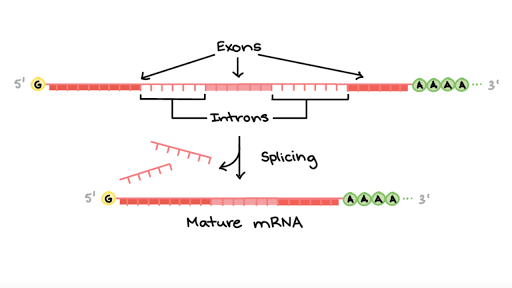
\includegraphics[width=6cm]{../figures/splicing_graphic.png} 
\label{fig:splicing}
\end{subfigure}
\begin{subfigure}{.5 \textwidth}
\centering
\caption{}  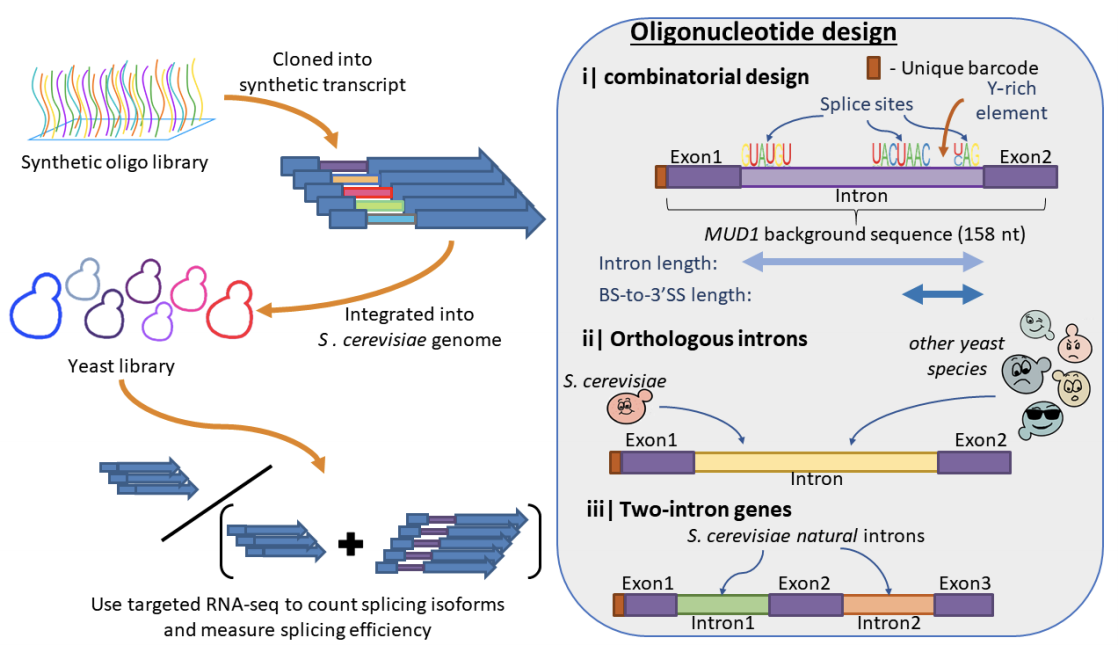
\includegraphics[width=6cm]{../figures/dataset_overview_pilpel.png} 
\label{fig:dataset}
\end{subfigure}
\caption{a) mRNA splicing overview. b) Schematic depicting the library of splicing efficiency measurements. Data and figure from Schirman, et al. bioRxiv 2021 \cite{pilpel}.}
\end{figure}
\subsection{Related work}
Large datasets have become available over the last decade that can aid in developing models predicting splicing efficiency from mRNA sequence. In some cases, splicing efficiency readouts have been obtained for designed libraries of thousands to millions of constructs (\cite{pilpel}, \cite{seelig}), and simple algorithms have achieved moderate predictive power for splicing efficiency (in the case of \cite{pilpel}, gradient boosting models with a small set of features achieves 0.77 Pearson correlation and in \cite{seelig}, a regression model explains 55-75\% of variation in splicing levels). Large collections of naturally occurring mRNA's have also been assayed, providing another opportunity for learning models to predict splicing efficiency. In SpanR, neural networks were trained based on feature sets with over 1000 hand-designed features, yielding an $R^2$ value of 0.65 between predicted and true splicing efficiency values \cite{spanr}. Deep learning approaches have already shown promise and enable splicing predictions without time-consuming hand-generation of features, with a 32-layer CNN SpliceAI successfully predicting a binary splicing or not splicing outcome given a position of interest and a large 10,000 sequence context \cite{spliceai}. Since RNN's have also shown some potential for predicting thermodynamic quantities based on RNA sequences \cite{rnn}, they could be useful for predicting splicing outcomes. However, deep learning approaches have not yet been used to predict continuous splicing efficiency values given an mRNA sequence, a prediction task critical for understanding downstream consequences of disease sequence variants.
\subsection{Contribution}
Here, we explore the ability of deep learning to predict the extent to which splicing happens at a particular position (value from 0 to 1) given varying windows in an mRNA sequence including both the intron and surrounding sequence, training models using a recently collected dataset of splicing efficiency values for tens of thousands of constructs in {\it Saccharomyces cerevisiae} (yeast). We compare a baseline model that uses simple sequence heuristics with CNN and RNN network architectures, and we analyze the network's error patterns and the features in the dataset used for prediction.

\section{Dataset and Features}
We use the dataset collected by Shirman, et al. \cite{pilpel} of splicing efficiency values for a library of 16268 designed sequence variants in yeast (Figure \ref{fig:dataset}). Each datapoint consists of a sequence of length 1615 nucleotides (A, C, T, or G) along with a corresponding splicing efficiency value (real values from 0 to 1), measured through RNA sequencing. The dataset consists of seven library types with different synthetic sequence design strategies to probe different backgrounds (12376 sequences) and five library types based on naturally occurring intron variants in {\it S. cerevisiae} and other related yeast species (3892 sequences).
\newline \\
To split the dataset into training, dev, and testing data, we used 90\% of each library type in the training set, and 5\% of each library type in the dev and test sets. By sampling these splits within library types, we ensured that the dev and test set have the same distribution. The original dataset contained the majority (80.3\%) of splicing efficiency values below 0.1; to correct this imbalance, we equalized the data between the ranges $[0, 0.1]$ and $[0.1, 1]$ by resampling. We made sure that near-identical sequences were not shared between the training, dev, and test sets. We explored approaches that made splicing efficiency predictions using: 1. the full 1615 nucleotide mRNA sequence, 2. the intron alone (maximum length 145 nucleotides), or 3. 20 nucleotide windows around three key splicing sequences in the mRNA (120 nucleotides total centered on the {\bf 5' splice site}, {\bf branch site}, and  {\bf 3' splice site} required for splicing \cite{splicingreview}).
\newline \\
TODO: Any diagrams of data

\section{ Methods }
\subsection{Baseline Model}
We first tested a baseline model using simple sequence heuristics to assign sequences to a splicing efficiency value. For each sequence in the dev set, we predicted its splicing efficiency value by comparing similarity to wildtype yeast mRNA that have introns that are spliced. If the sequence is not similar to known spliced mRNA's in yeast, we predict a splicing efficiency of 0, and if it is similar, we assign the predicted splicing efficiency value to be  the average splicing efficiency value from the training set (computed using only sequences with splicing level above $\epsilon = 0.001$). \newline \\
To evaluate similarity of sequences in the dev set to wildtype yeast spliced mRNA's we used the following heuristics. At a first approximation, splicing occurs when the cell's splicing machinery recognizes three short key sequences in mRNAs: the 5' splice site (6 nucleotides at the start of an intron), branch site (8 nucleotides in the latter portion of the intron), and 3' splice site (3 nucleotides at the end of the intron) \cite{splicingreview}. First we compute the position weight matrix (nucleotide distribution) for sequence motifs at each of these three key sequences using wildtype yeast mRNAs. We additionally compute two length distributions from wildtype introns: the full length of the intron, and the length between the branch site and 3' splice site. For a tested sequence to be marked as similar to wildtype yeast splicing mRNA's, we require that sequences' score against the position weight matrix and length distributions fall within the 95th percentile of wildtype introns.
\subsection{RNN Model}
LSTM models have been shown to capture long-range base-pairing interactions in RNA sequences \cite{rnn}, which play a role in regulating mRNA splicing efficiency. These long-range interactions represent second-order effects that would not be captured by the baseline model. We implemented a bidirectional LSTM architecture consisting of a first convolutional layer (64 filters, kernel size of 15 and stride-length of 4) followed by a dropout layer, two bidirectional LSTM layers with dropout and batch normalization layers, and a final set of dense layers with ReLU activations.
\subsection{CNN Model}
CNN models have been used fruitfully to predict binary splicing outcomes from mRNA sequence \cite{spliceai}. We trained CNN models with residual blocks to facilitate useful gradient updates, with each residual block including convolution layers, batch normalization layers, and ReLU activations (Figure . The final layer of the CNN architectures was a dense layer with a ReLU activation. We explored architectures with varying numbers of residual blocks (one or four), removing add blocks (leaving only convolutional layers), varying the presence of a convolutional layer after the residual block, and varying the amount of sequence context used for prediction. The parameters for filter size, stride length, and number of filters were obtained from the CNN's trained in \cite{spliceai}.
\subsection{Training strategy and evaluation metrics}
Since we are predicting a real-valued outcome, we use a mean-squared error regression loss function as implemented in Keras, and we will use a ReLU activation function for the final node in the neural network models. We tuned hyperparameters by evaluating them on the dev dataset, and we evaluate the final models on the test dataset. We trained the RNN and CNN models over 20 epochs using Adam optimization with mini-batches, and we used early stopping for regularization, monitoring the validation loss and ending training after two consecutive epochs with a change in loss of less than 0.001. For each architecture choice, we chose the best of 5 models trained with different random weight initializations. 
\subsection{Implementation} 
All deep learning methods were implemented in Keras using TensorFlow 2.0, with logging through wandb and model interpretation through \texttt{tf\_keras\_vis}. Code is available at \texttt{https://github.com/ramyarangan/cs230\_project}.

\begin{figure}[H]
\centering
\begin{subfigure}{.2 \textwidth}
\centering
\caption{} 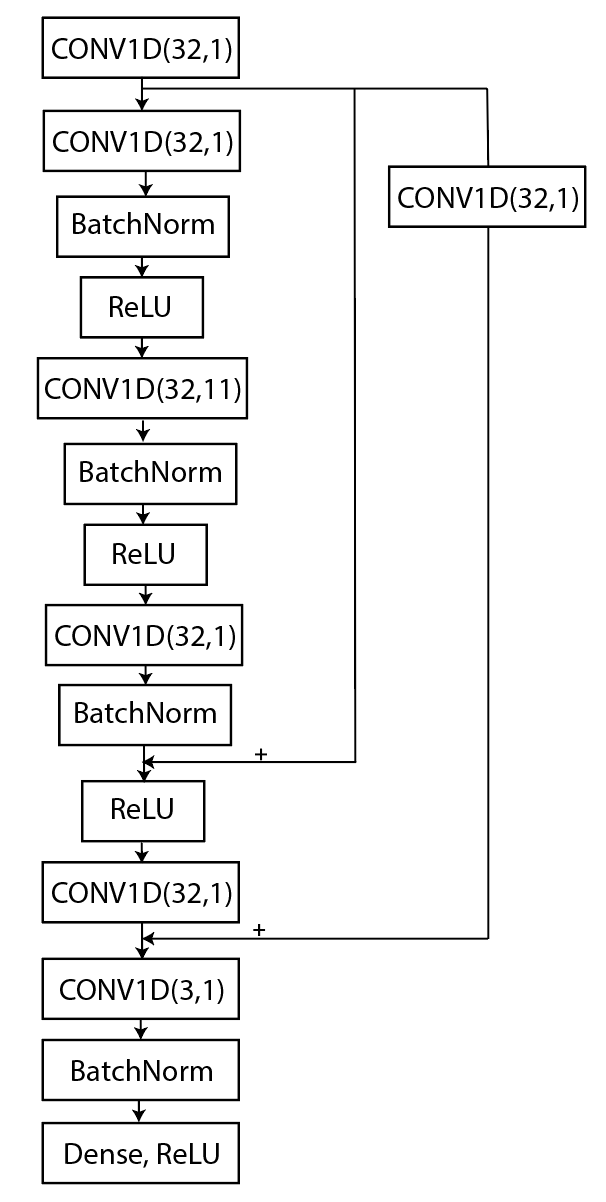
\includegraphics[width=4cm]{../figures/cnn_architecture.png} 
\label{fig:architecture}
\end{subfigure}
\begin{subfigure}{.7 \textwidth}
\centering
\caption{}  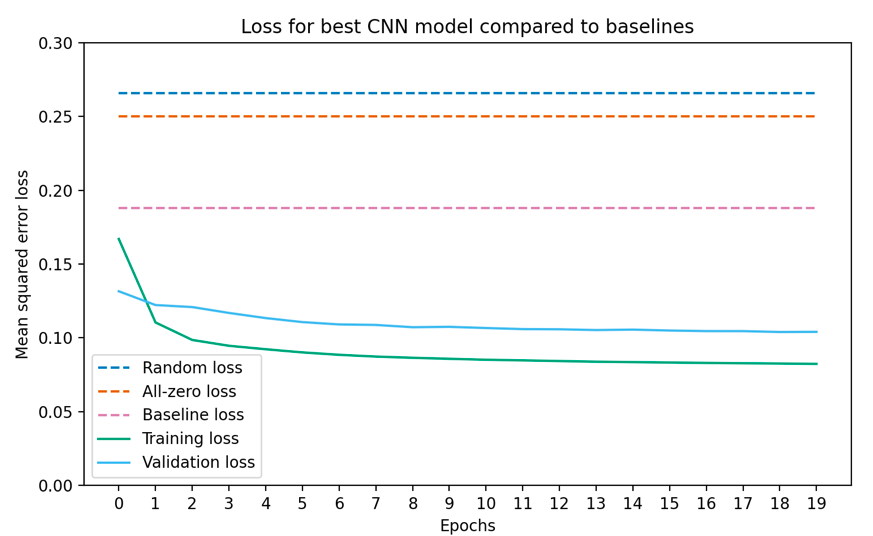
\includegraphics[width=8cm]{../figures/loss.png} 
\label{fig:loss}
\end{subfigure}
\caption{a) CNN architecture for best network. b) Mean-squared error loss over epochs of training for best network.}
\end{figure}

\section{Experiments and Results}
\subsection{Hyper-parameter exploration}
To decide on hyper-parameters of the network, for the CNN architecture with 4 residual blocks trained on a 120 nucleotide window of sequence data, we varied learning rates (0.01, 0.001, and 0.0001), mini-batch sizes (32, 64, 128), and the momentum parameters (0.9 and 0.95). We found that we were able to achieve the best performance on the validation set for this CNN architecture with a learning rate $\alpha = 0.001$, momentum $\beta_1 = 0.9$, and mini-batch size of 64. We additionally chose standard values of $\beta_2 = 0.999$ and the decay value of $0.01$ for Adam optimization. 
\subsection{Model performance} 
When the Baseline Model is used to predict splicing efficiency values for the development set, the mean-squared error loss on the dev set is {\bf 0.0638}, compared to the mean-squared error loss of {\bf 0.308} for a random model that predicts uniform random values from 0 to 1 for all dev set examples.
\subsection{Error analysis and interpretation}

What your primary metrics are: accuracy, precision,
AUC, etc. Provide equations for the metrics if necessary. For results, you want to have a
mixture of tables and plots. If you are solving a classification problem, you should include a
confusion matrix or AUC/AUPRC curves. Include performance metrics such as precision,
recall, and accuracy. For regression problems, state the average error. You should have
both quantitative and qualitative results. To reiterate, you must have both quantitative
and qualitative results! If it applies: include visualizations of results, heatmaps,
examples of where your algorithm failed and a discussion of why certain algorithms failed
or succeeded. In addition, explain whether you think you have overfit to your training set
and what, if anything, you did to mitigate that. Make sure to discuss the figures/tables in
your main text throughout this section. Your plots should include legends, axis labels, and
have font sizes that are legible when printed.

\section{Conclusion/Future Work }
Model size given data, SpliceAI work comparison. 
Summarize your report and reiterate key points. Which algorithms were the highestperforming?
Why do you think that some algorithms worked better than others? For
future work, if you had more time, more team members, or more computational resources,
what would you explore?
We can augment the training dataset with additional negative examples by using intervals from the yeast genome that do not overlap with naturally occurring spliced mRNA's, assigning these examples to the splicing efficiency value of 0. 

\section{Contributions}
The contributions section is not included in the 5 page limit. This section should describe
what each team member worked on and contributed to the project.

\section*{References}
This section should include citations for: (1) Any papers mentioned in the related work
section. (2) Papers describing algorithms that you used which were not covered in class.
(3) Code or libraries you downloaded and used. This includes libraries such as scikit-learn, Tensorflow, Pytorch, Keras etc. Acceptable formats include: MLA, APA, IEEE. If you
do not use one of these formats, each reference entry must include the following (preferably
in this order): author(s), title, conference/journal, publisher, year. If you are using TeX,
you can use any bibliography format which includes the items mentioned above. We are excluding
the references section from the page limit to encourage students to perform a thorough
literature review/related work section without being space-penalized if they include more
references. Any choice of citation style is acceptable
as long as you are consistent. 


\begin{thebibliography}{9}
\bibitem{pilpel} 
Schirman, D., Yakhini, Z., Dahan, O., Pilpel, Y.
\textit{Sequence determinants and evolution of constitutive and alternative splicing in yeast species}. 2021. bioRxiv. 

\bibitem{seelig} 
Rosenberg, A.B., Patwardhan, R.P., Shendure, J., Seelig, G.
\textit{Learning the sequence determinants of alternative splicing from millions of random sequences.}. 2015. Cell, 163 (698-711). 

\bibitem{spanr}
Xiong, H.Y., Alipanahi, B., Lee, L.J., et al. 
\textit{The human splicing code reveals new insights into the genetic determinants of disease.} 2015. Science, 347 (1254806).

\bibitem{spliceai} 
Jaganathan, K., Panagiotopoulou, S. K., McRae, J.F., et al. 
\textit{Predicting splicing from primary Sequence with deep learning}. 2019. Cell, 176 (535-548). 

\bibitem{rnn} 
Wu, M., Andreasson, J.O.L, Kladwang, W., et al. \textit{Prospects for recurrent neural network models to learn RNA
biophysics from high-throughput data}. 2018. bioRxiv.

\bibitem{splicingreview}
Wilkinson, M.E., Charenton, C., Nagai, K. \textit{RNA Splicing by the Spliceosome}. 2019. Annual Review of Biochemistry, 89 (359-388).

\end{thebibliography}


\end{document}